\chapter{Configuration et maintenance de \ReplicaNextLong{}}\label{ch:replica-next-setup}

Cette section s'applique au tableau \ReplicaNextLong{} illustré à l'\autoref{fig:next-hardware}.

\begin{figure}[htbp]
    \centering
    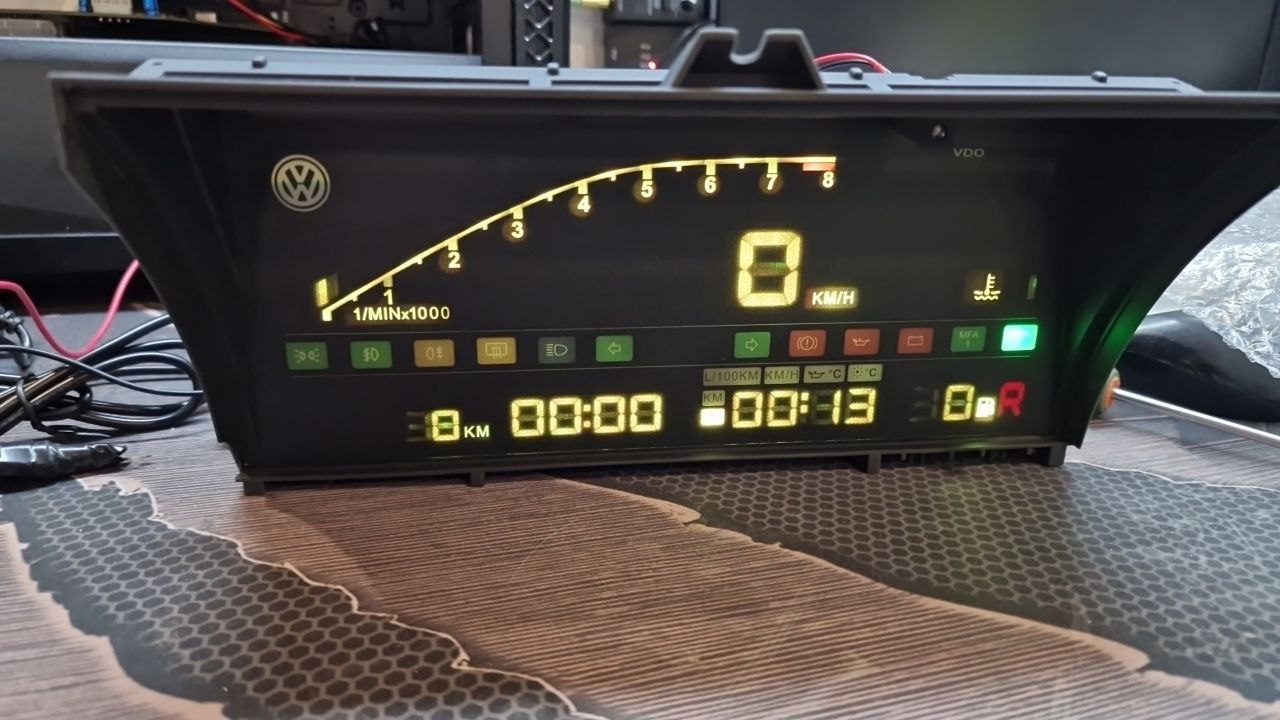
\includegraphics[width=0.6\textwidth]{digifiz_manual/image019.png}
    \caption{Assemblage du tableau \ReplicaNextLong{}.}
    \label{fig:next-hardware}
\end{figure}

\section{Manipulation du combiné}
\begin{itemize}
    \item La façade en polycarbonate imprimée aux UV doit être protégée des rayures et corps étrangers. Toute détérioration importante nécessite des pièces de rechange auprès de PHOL-LABS Kft et n'est pas couverte par la garantie.
    \item L'horloge temps réel se règle via le portail Wi-Fi. Elle se réinitialise dès que l'alimentation permanente est coupée.
\end{itemize}

\section{Portail de contrôle Wi-Fi}
La configuration, la collecte de données et la gestion du micrologiciel s'effectuent via l'application web embarquée.
\begin{itemize}
    \item Connectez-vous au point d'accès Wi-Fi du tableau. Désactivez les données mobiles et rejoignez \texttt{Digifiz\_AP} (mot de passe \texttt{87654321}); certaines révisions annoncent \texttt{PHOL-LABS2} avec le même mot de passe.
    \item L'adresse IP par défaut est \texttt{192.168.4.1}. Si le tableau est configuré pour rejoindre un autre réseau, analysez le sous-réseau à la recherche d'une adresse se terminant par \texttt{.32} à l'aide d'un utilitaire IP.
    \item Le portail comporte cinq onglets~: \emph{WiFi}, \emph{Control}, \emph{Settings}, \emph{Colors} et \emph{About} (\autoref{fig:next-control-tabs}). L'onglet WiFi gère les paramètres réseau et les mises à jour de micrologiciel ; l'onglet Control ajuste les paramètres du tableau ; l'onglet Settings propose un éditeur structuré de tous les paramètres du micrologiciel ; l'onglet Colors pilote les jeux de couleurs multi-segments ; l'onglet About récapitule les informations sur les auteurs.
\end{itemize}

\begin{figure}[htbp]
    \centering
    \begin{subfigure}{0.48\textwidth}
        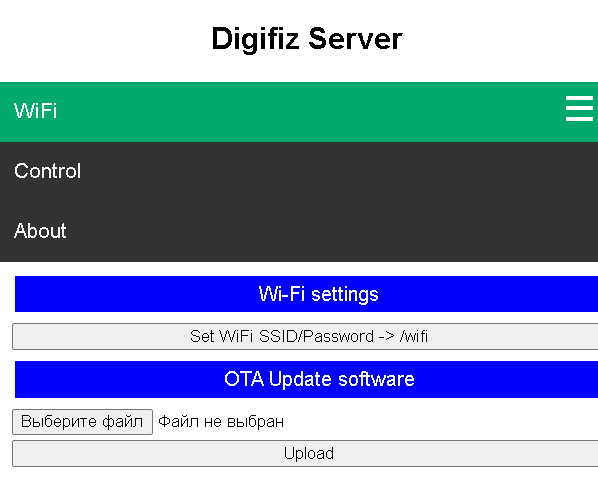
\includegraphics[width=\linewidth]{digifiz_manual/image020.png}
        \caption{Vue d'ensemble de l'onglet Control.}
    \end{subfigure}\hfill
    \begin{subfigure}{0.48\textwidth}
        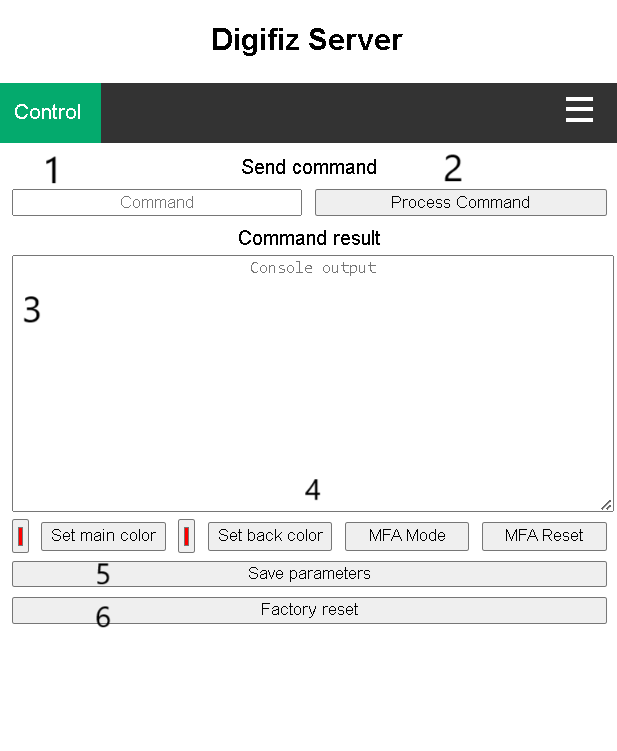
\includegraphics[width=\linewidth]{digifiz_manual/image021.png}
        \caption{Commandes numérotées et zones de saisie.}
    \end{subfigure}
    \caption{Interface Wi-Fi de \ReplicaNextShort{}.}
    \label{fig:next-control-tabs}
\end{figure}

\section{Saisie de commandes}
L'onglet \emph{Control} met à disposition une ligne de commande (1), un bouton \emph{Process} (2), une fenêtre de résultat (3), des réglages rapides (4), un bouton \emph{Save} (5) et un bouton \emph{Reset} (6).
Saisissez les commandes sous la forme de paires séparées par un espace \verb|<numéro> <valeur>| en utilisant uniquement des entiers ; la ponctuation et les guillemets sont inutiles.
L'\autoref{fig:next-command-example} illustre l'interface lors de la désactivation du réglage automatique de luminosité.

\begin{figure}[htbp]
    \centering
    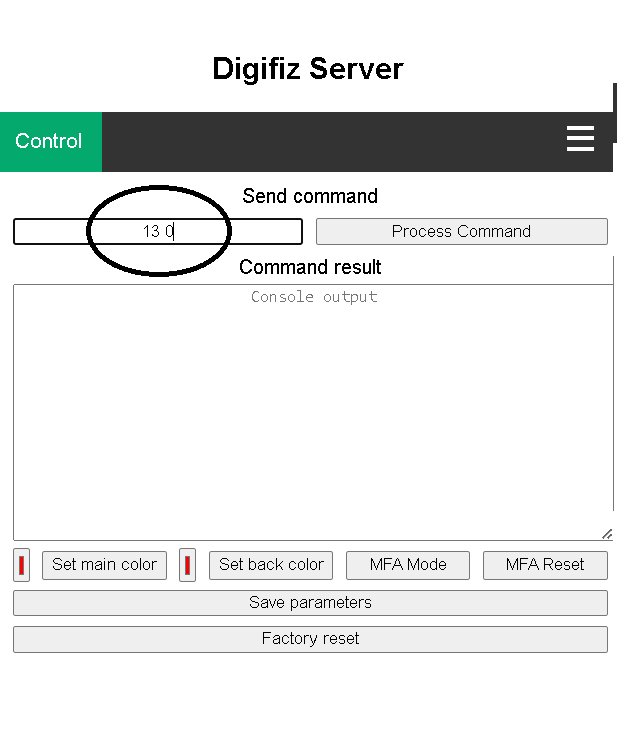
\includegraphics[width=0.55\textwidth]{digifiz_manual/image022.png}
    \caption{Exemple de commande désactivant la luminosité automatique.}
    \label{fig:next-command-example}
\end{figure}

\section{Référence de commandes}
\begin{table}[htbp]
    \centering
    \caption{Commandes principales de configuration \ReplicaNextShort{}.}
    \label{tbl:next-commands}
    {\scriptsize
    \begin{tblr}{
        colspec = {Q[c,0.14\linewidth] Q[l,0.36\linewidth] Q[l]},
        rowsep = 2pt,
    }
        \toprule
        \textbf{Commande} & \textbf{Nom} & \textbf{Description} \\
        \midrule
        22 (ou 0) & \paramname{PARAMETER\_RPMCOEFFICIENT} & Facteur d'étalonnage du régime (100--10000). \\
        1  & \paramname{PARAMETER\_SPEEDCOEFFICIENT} & Facteur d'étalonnage de vitesse (10--255). \\
        2  & \paramname{PARAMETER\_COOLANTTHERMISTORB} & Coefficient bêta de la sonde de liquide (2000--5000). \\
        3  & \paramname{PARAMETER\_OILTHERMISTORB} & Coefficient bêta de la sonde d'huile (2000--5000). \\
        4  & \paramname{PARAMETER\_AIRTHERMISTORB} & Coefficient bêta de la sonde ambiante (2000--5000). \\
        5  & \paramname{PARAMETER\_TANKMINRESISTANCE} & Résistance minimale de jauge (0--1000~\ohm). \\
        6  & \paramname{PARAMETER\_TANKMAXRESISTANCE} & Résistance maximale de jauge (100--1000~\ohm). \\
        7  & \paramname{PARAMETER\_TAU\_COOLANT} & Constante de filtrage température liquide (1--50, plus haut = plus réactif). \\
        8  & \paramname{PARAMETER\_TAU\_OIL} & Constante de filtrage température huile (1--50). \\
        9  & \paramname{PARAMETER\_TAU\_AIR} & Constante de filtrage température ambiante (1--50). \\
        10 & \paramname{PARAMETER\_TAU\_TANK} & Constante de filtrage niveau carburant (1--50). \\
        11 & \paramname{PARAMETER\_MILEAGE} & Kilométrage total (0--999999). \\
        12 & \paramname{PARAMETER\_DAILY\_MILEAGE} & Compteur journalier (0--9999). \\
        13 & \paramname{PARAMETER\_AUTO\_BRIGHTNESS} & Activation de la luminosité automatique (1=actif, 0=inactif). \\
        14 & \paramname{PARAMETER\_BRIGHTNESS\_LEVEL} & Niveau de luminosité manuelle (0--60~\%; >60 réduit la durée de vie des LED). \\
        15 & \paramname{PARAMETER\_TANK\_CAPACITY} & Capacité du réservoir en litres (0--99 ; 55~L typique pour Golf~2). \\
        16 & \paramname{PARAMETER\_MFA\_STATE} & Mode MFA actif (normalement piloté par l'entrée matérielle). \\
        17 & \paramname{PARAMETER\_BUZZER\_OFF} & Désactivation du buzzer (1 coupe, 0 active ; \ReplicaNextShort{} n'intègre pas de buzzer). \\
        18 & \paramname{PARAMETER\_MAX\_RPM} & Échelle du compte-tours (8000 typique, plage 4000--16000). \\
        19 & \paramname{PARAMETER\_NORMAL\_RESISTANCE\_COOLANT} & Résistance de sonde liquide à \SI{25}{\celsius} (1000--10000~\ohm). \\
        20 & \paramname{PARAMETER\_NORMAL\_RESISTANCE\_OIL} & Résistance de sonde huile à \SI{25}{\celsius} (1000--10000~\ohm). \\
        21 & \paramname{PARAMETER\_NORMAL\_RESISTANCE\_AMB} & Résistance de sonde ambiante à \SI{25}{\celsius} (1000--10000~\ohm). \\
        23 & \paramname{PARAMETER\_DOT\_OFF} & Comportement des deux-points de l'horloge (0=clignotant, 1=fixe). \\
        24 & \paramname{PARAMETER\_BACKLIGHT\_ON} & Activation du rétroéclairage avec les feux de croisement (non utilisé sur \ReplicaNextShort{}). \\
        25 & \paramname{PARAMETER\_M\_D\_FILTER} & Constante de filtre médian (héritage, généralement inutilisée). \\
        26 & \paramname{PARAMETER\_COOLANT\_MAX\_R} & Seuil de sonde liquide pour affichage pleine échelle (\SI{100}{\celsius}--\SI{150}{\celsius}). \\
        27 & \paramname{PARAMETER\_COOLANT\_MIN\_R} & Seuil de sonde liquide pour indication « 1~bar » (\SI{0}{\celsius}--\SI{80}{\celsius}). \\
        31 & \paramname{PARAMETER\_MAINCOLOR\_R} & Composante rouge de l'interface (0--255). \\
        32 & \paramname{PARAMETER\_MAINCOLOR\_G} & Composante verte de l'interface (0--255). \\
        33 & \paramname{PARAMETER\_MAINCOLOR\_B} & Composante bleue de l'interface (0--255). \\
        37 & \paramname{PARAMETER\_RPM\_FILTER} & Réactivité du filtre régime (10--200, plus haut = plus rapide). \\
        128 & \paramname{PARAMETER\_READ\_ADDITION} & Ajouter 128 pour lire la valeur courante d'une commande. \\
        255 & \paramname{PARAMETER\_SET\_HOUR} & Réglage des heures (format 24~h). \\
        254 & \paramname{PARAMETER\_SET\_MINUTE} & Réglage des minutes. \\
        253 & \paramname{PARAMETER\_RESET\_DAILY\_MILEAGE} & Remise à zéro du compteur journalier. \\
        252 & \paramname{PARAMETER\_RESET\_DIGITAL} & Réinitialisation usine des paramètres stockés. \\
        \bottomrule
    \end{tblr}}
\end{table}

\section{Valeurs par défaut}
\begin{table}[htbp]
    \centering
    \caption{Paramètres par défaut \ReplicaNextShort{}.}
    \label{tbl:next-defaults}
    {\scriptsize
    \begin{tblr}{
        colspec = {Q[l,0.42\linewidth] Q[c,0.15\linewidth] Q[l]},
        rowsep = 2pt,
    }
        \toprule
        \textbf{Paramètre} & \textbf{Valeur} & \textbf{Remarques} \\
        \midrule
        \paramname{PARAMETER\_RPMCOEFFICIENT} & 3000 & Typique pour les entrées compte-tours Audi. \\
        \paramname{PARAMETER\_SPEEDCOEFFICIENT} & 100 & Étalloné pour 100~km/h. \\
        \paramname{PARAMETER\_COOLANTTHERMISTORB} & 4000 &  \\
        \paramname{PARAMETER\_OILTHERMISTORB} & 4000 &  \\
        \paramname{PARAMETER\_AIRTHERMISTORB} & 3812 & 3600 pour les panneaux génération~2. \\
        \paramname{PARAMETER\_TANKMINRESISTANCE} & 35 & \ohm. \\
        \paramname{PARAMETER\_TANKMAXRESISTANCE} & 265 & \ohm. \\
        \paramname{PARAMETER\_TAU\_COOLANT} & 2 & Constante de filtre. \\
        \paramname{PARAMETER\_TAU\_OIL} & 2 & Constante de filtre. \\
        \paramname{PARAMETER\_TAU\_AIR} & 2 & Constante de filtre. \\
        \paramname{PARAMETER\_TAU\_TANK} & 2 & Constante de filtre. \\
        \paramname{PARAMETER\_MILEAGE} & Spécifique au véhicule & Conserve l'odomètre stocké. \\
        \paramname{PARAMETER\_DAILY\_MILEAGE} & 0 &  \\
        \paramname{PARAMETER\_AUTO\_BRIGHTNESS} & 1 & Activée. \\
        \paramname{PARAMETER\_BRIGHTNESS\_LEVEL} & 25 & Valeur par défaut génération~2 ; génération~1/1.5~: 7 ou 13. \\
        \paramname{PARAMETER\_TANK\_CAPACITY} & 63 & Litres. \\
        \paramname{PARAMETER\_MFA\_STATE} & 0 & Page MFA par défaut. \\
        \paramname{PARAMETER\_BUZZER\_OFF} & 1 & Buzzer désactivé. \\
        \paramname{PARAMETER\_MAX\_RPM} & 8000 & Échelle du compte-tours. \\
        \paramname{PARAMETER\_NORMAL\_RESISTANCE\_COOLANT} & 1000 & \ohm{} à \SI{25}{\celsius}. \\
        \paramname{PARAMETER\_NORMAL\_RESISTANCE\_OIL} & 1000 & \ohm{} à \SI{25}{\celsius}. \\
        \paramname{PARAMETER\_NORMAL\_RESISTANCE\_AMB} & 2991 & 500~\ohm{} pour les sondes génération~2. \\
        \paramname{PARAMETER\_DOT\_OFF} & 0 & Deux-points clignotant. \\
        \paramname{PARAMETER\_BACKLIGHT\_ON} & 1 & Rétroéclairage actif avec les feux de croisement. \\
        \paramname{PARAMETER\_M\_D\_FILTER} & 65535 & Constante historique de filtre médian. \\
        \paramname{PARAMETER\_COOLANT\_MAX\_R} & 120 & \si{\celsius}. \\
        \paramname{PARAMETER\_COOLANT\_MIN\_R} & 60 & \si{\celsius}. \\
        \paramname{PARAMETER\_MAINCOLOR\_R} & 180 & Défaut jaune-vert. \\
        \paramname{PARAMETER\_MAINCOLOR\_G} & 240 & Défaut jaune-vert. \\
        \paramname{PARAMETER\_MAINCOLOR\_B} & 6 & Défaut jaune-vert. \\
        \paramname{PARAMETER\_RPM\_FILTER} & 70 & Réponse du filtre. \\
        \paramname{PARAMETER\_UPTIME} & 0 & Compteur de fonctionnement. \\
        \bottomrule
    \end{tblr}}
\end{table}

\section{Lecture des paramètres et exemples}
Pour lire un paramètre, ajoutez 128 au numéro de commande (par exemple \verb|129 0| retourne le facteur de vitesse).
Parmi les commandes courantes~: désactiver la luminosité automatique (\verb|13 0|), la réactiver (\verb|13 1|), ajuster le facteur de vitesse (\verb|1 110| augmente l'affichage de 10~\%) et définir l'odomètre (\verb|11 123456|).
L'horloge se règle avec \verb|255 <heures>| puis \verb|254 <minutes>|.
Les commandes 31 à 33 fixent les composantes RVB de la couleur d'interface.

\section{Commandes de service}
Les versions récentes du micrologiciel acceptent les noms de paramètres lisibles, par exemple \verb|PARAMETER_RPMCOEFFICIENT 3000|.
La commande de diagnostic \verb|adc 0| affiche les mesures ADC brutes pour le dépannage des capteurs.
Les mises à jour de micrologiciel ajoutent des contrôles visuels de couleur ; mettez régulièrement à jour via l'onglet \emph{WiFi} pour profiter des dernières fonctionnalités.

\section{Éditeur de paramètres (onglet Settings)}
L'onglet \emph{Settings} reprend la liste de \autoref{tbl:next-commands} et \autoref{tbl:next-defaults} en y ajoutant les plages autorisées, le type de donnée et des infobulles.
Il constitue une alternative graphique à la saisie de commandes numériques.

\begin{enumerate}
    \item Cliquez sur \emph{Load Parameters} pour charger les valeurs en direct depuis le tableau. Chaque ligne affiche le nom du paramètre, sa valeur courante, une description et son type.
    \item Pour les champs numériques, saisissez la valeur souhaitée dans la colonne \emph{New Value}. L'interface impose la plage indiquée dans les colonnes \emph{Min} et \emph{Max}. Les paramètres booléens sont présentés sous forme de cases à cocher.
    \item Appuyez sur \emph{Set} pour envoyer immédiatement la modification. Le tableau se recharge afin de confirmer la mise à jour.
    \item Répétez l'opération pour chaque paramètre à ajuster. Une fois terminé, revenez dans l'onglet \emph{Control} et appuyez sur \emph{Save parameters} afin d'écrire la configuration en mémoire non volatile.
\end{enumerate}

Avant d'utiliser l'onglet \emph{Colors}, activez l'indicateur micrologiciel dédié aux palettes personnalisées.
Repérez la case booléenne intitulée «~Custom colour scheme~» (exposée sous la forme \verb|PARAMETER_CUSTOM_COLORSCHEME_ENABLE| dans la liste) ; cochez-la puis validez avec \emph{Set}. Le tableau refusera toute modification de segments tant que ce drapeau reste inactif.

\section{Jeux de couleurs personnalisés}
L'onglet \emph{Colors} fournit un éditeur par segments pour le rétroéclairage WS2812. Chaque ligne définit une fin de plage, la zone fonctionnelle concernée et la couleur (fixe ou héritée).

\begin{enumerate}
    \item Cliquez sur \emph{Load Scheme} pour lire la cartographie active. Utilisez \emph{Add Segment} ou les contrôles «~+\textuparrow{}~» et «~+\textdownarrow{}~» pour insérer de nouvelles plages. Les listes déroulantes associent la fonction instrument, tandis que le sélecteur de base permet de réemployer la couleur principale ou d'arrière-plan plutôt qu'un RVB fixe.
    \item Ajustez la teinte via le sélecteur de couleur pour les segments configurés en «~Custom~». L'éditeur affiche en direct les composantes.
    \item Réordonnez les lignes à l'aide des flèches afin de respecter l'ordre physique des LED (les segments doivent rester croissants). Supprimez les entrées inutiles avec le bouton «~\texttimes{}~».
    \item Lorsque la table reflète le rendu souhaité, appuyez sur \emph{Set Scheme}. Le navigateur parcourt chaque segment et l'envoie au tableau.
    \item Passez immédiatement dans l'onglet \emph{Control} et cliquez sur \emph{Save parameters}. Cette étape est obligatoire~: sans sauvegarde, le micrologiciel conserve les segments en RAM et les perdra après redémarrage.
    \item Exportez éventuellement la représentation JSON via \emph{Export to File} pour constituer une sauvegarde, ou importez un fichier existant avec \emph{Import from File}. Le bouton \emph{Reset Scheme} restaure la configuration d'usine après confirmation.
\end{enumerate}

Si vous désactivez ultérieurement le drapeau de jeu de couleurs personnalisé dans l'onglet \emph{Settings}, le tableau revient au mode monochrome classique piloté par \verb|PARAMETER_MAINCOLOR_R/G/B|.
